%%%%%%%%%%%%%%%%%%%%%%%%%%%%%%%%%%%%%%%%%
% Short Sectioned Assignment
% LaTeX Template
% Version 1.0 (5/5/12)
%
% This template has been downloaded from:
% http://www.LaTeXTemplates.com
%
% Original author:
% Frits Wenneker (http://www.howtotex.com)
%
% License:
% CC BY-NC-SA 3.0 (http://creativecommons.org/licenses/by-nc-sa/3.0/)
%
%%%%%%%%%%%%%%%%%%%%%%%%%%%%%%%%%%%%%%%%%

%----------------------------------------------------------------------------------------
%	PACKAGES AND OTHER DOCUMENT CONFIGURATIONS
%----------------------------------------------------------------------------------------

\documentclass[paper=a4, fontsize=11pt]{scrartcl} % A4 paper and 11pt font size

\usepackage[T1]{fontenc} % Use 8-bit encoding that has 256 glyphs
\usepackage{fourier} % Use the Adobe Utopia font for the document - comment this line to return to the LaTeX default
\usepackage[english]{babel} % English language/hyphenation
\usepackage{amsmath,amsfonts,amsthm, amssymb} % Math packages
\usepackage{enumitem}
\usepackage{cancel}
\usepackage{graphicx} % Required to insert images
\usepackage{color}
\definecolor{dkgreen}{rgb}{0,0.6,0}
\definecolor{gray}{rgb}{0.5,0.5,0.5}
\definecolor{mauve}{rgb}{0.58,0,0.82}
\usepackage{listings}
\lstset{frame=tb,
  language=Python,
  aboveskip=3mm,
  belowskip=3mm,
  showstringspaces=false,
  columns=flexible,
  basicstyle={\small\ttfamily},
  numbers=none,
  numberstyle=\tiny\color{gray},
  keywordstyle=\color{blue},
  commentstyle=\color{dkgreen},
  stringstyle=\color{mauve},
  breaklines=true,
  breakatwhitespace=true
  tabsize=3
}
\usepackage{pgfplotstable}% For inserting csv table

\usepackage{sectsty} % Allows customizing section commands
\allsectionsfont{\centering \normalfont\scshape} % Make all sections centered, the default font and small caps

\usepackage{fancyhdr} % Custom headers and footers
\pagestyle{fancyplain} % Makes all pages in the document conform to the custom headers and footers
\fancyhead{} % No page header - if you want one, create it in the same way as the footers below
\fancyfoot[L]{} % Empty left footer
\fancyfoot[C]{} % Empty center footer
\fancyfoot[R]{\thepage} % Page numbering for right footer
\renewcommand{\headrulewidth}{0pt} % Remove header underlines
\renewcommand{\footrulewidth}{0pt} % Remove footer underlines
\setlength{\headheight}{13.6pt} % Customize the height of the header

\numberwithin{equation}{section} % Number equations within sections (i.e. 1.1, 1.2, 2.1, 2.2 instead of 1, 2, 3, 4)
\numberwithin{figure}{section} % Number figures within sections (i.e. 1.1, 1.2, 2.1, 2.2 instead of 1, 2, 3, 4)
\numberwithin{table}{section} % Number tables within sections (i.e. 1.1, 1.2, 2.1, 2.2 instead of 1, 2, 3, 4)

\setlength\parindent{0pt} % Removes all indentation from paragraphs - comment this line for an assignment with lots of text

%----------------------------------------------------------------------------------------
%	TITLE SECTION
%----------------------------------------------------------------------------------------

\newcommand{\horrule}[1]{\rule{\linewidth}{#1}} % Create horizontal rule command with 1 argument of height

\title{	
\normalfont \normalsize 
\textsc{Baruch, MFE} \\ [25pt] % Your university, school and/or department name(s)
\horrule{0.5pt} \\[0.4cm] % Thin top horizontal rule
\huge MTH 9876 Assignment One\\  % The assignment title
\horrule{2pt} \\[0.5cm] % Thick bottom horizontal rule
}


\author{Zhou, ShengQuan} % Your name

\date{\normalsize\today} % Today's date or a custom date

\begin{document}
	


\maketitle % Print the title

\newpage



\section{Loss Given Default}
Loss given default (LGD) is a measure of the severity of a default, and is
defined as the fraction of the face value of a bond that is not repaid to the
investor. In other words,
$$
\text{LGD} = (1-R)\times F.
$$
\textbf{(i)} Find the probability distribution of LGD in Merton's model.\\
\textit{Solution}: Given the occurrence of a default at time $T$, 
the amount paid to the investor is the value of the firm $V_T$. Thus,
the fraction of the face value of a bond that is not repaid to the investor is
\begin{align}
\nonumber \text{LGD} &\triangleq F(1-R) = \left(F - V_T\right)^+,
\end{align}
By definition, $0\le \text{LGD} < F$. Let $0\le x< F$,
\begin{align}
\nonumber \mathbb{P}\left(\text{LGD}<x\right) &= \mathbb{P}\left(F - V_T\le x | V_T<F \right)\mathbb{P}\left(V_T<F\right)+\mathbb{P}\left(V_T\ge F\right)\\
\nonumber &= \mathbb{P}\left(F-x\le V_T<F\right)+\mathbb{P}\left(V_T\ge F\right)\\
\nonumber &=\mathbb{P}\left(V_T\ge F-x\right).
\end{align}
Invoking the well-known formula for the risk-neutral survival probability with face value $F$,
$$
\mathbb{P}\left(V_T\ge F\right) = N(d_-)
$$
where
$$
d_- \triangleq \frac{1}{\sigma_V\sqrt{T}}\left[ \log\frac{V_0}{F} + \left(r -\frac{1}{2}\sigma_V^2\right)T \right],
$$
the cumulative distribution function of LGD can be written as
\begin{align}
\nonumber \mathbb{P}\left(\text{LGD}<x\right) &= N\left(d_-(x)\right),
\end{align}
where $d_-(x)$ is obtained by replacing $F$ by $F-x$ in $d_-$, such that $d_-(0)=d_-$:
$$
d_-(x) \triangleq \frac{1}{\sigma_V\sqrt{T}}\left[ \log\frac{V_0}{F-x} + \left(r -\frac{1}{2}\sigma_V^2\right)T \right].
$$
The density function is obtained by differentiating $\mathbb{P}\left(\text{LGD}<x\right)$ with respect to $x$, for $0\le x<F$,
\begin{align}
\nonumber f_{\text{LGD}}(x) &= \frac{\partial}{\partial x}\mathbb{P}\left(\text{LGD}<x\right) \\
\nonumber &= \frac{1}{\sqrt{2\pi}}e^{-\frac{d_-(x)^2}{2}}\frac{\partial d_-(x)}{\partial x}  + N\left(d_-\right)\delta(x)\\
\nonumber &= \frac{e^{-\frac{d_-(x)^2}{2}}}{\sigma_V\sqrt{2\pi T}(F-x)} + N\left(d_-\right)\delta(x).
\end{align} 
For $x<0$, we have $f_{\text{LGD}}(x) = 0$. Notice that there is a Dirac-$\delta$ component in the probability density function because at $x=0$, the cumulative distribution 
function is discontinuous:
\begin{align}
\nonumber \mathbb{P}\left(\text{LGD}<0\right) &=0,\\
\nonumber \mathbb{P}\left(\text{LGD}\le 0\right) & = N(d_-).
\end{align}
The above discontinuity is caused by the fact that the finite probability $N(d_-)$ of the equity value ending up with $V_T>F$ contributes
to the isolated point of zero LGD.\\

(ii) Implement the formula for the density function and plot it for $T = 10
$ and $V_0 = 95, 99, 120, 140$ (as usual, $F = 100$).\\
\textit{Solution}: We choose $\sigma_V = 30\%$ and $r=0.1\%$. The singular components corresponding to the Dirac-$\delta$ 
located at $x=0$ are not depicted in graph. This example indicates that, given default, the most probable recovery rate falls in the approximate range of $R^*\in [20\%, 40\%]$.
\begin{figure}[h]
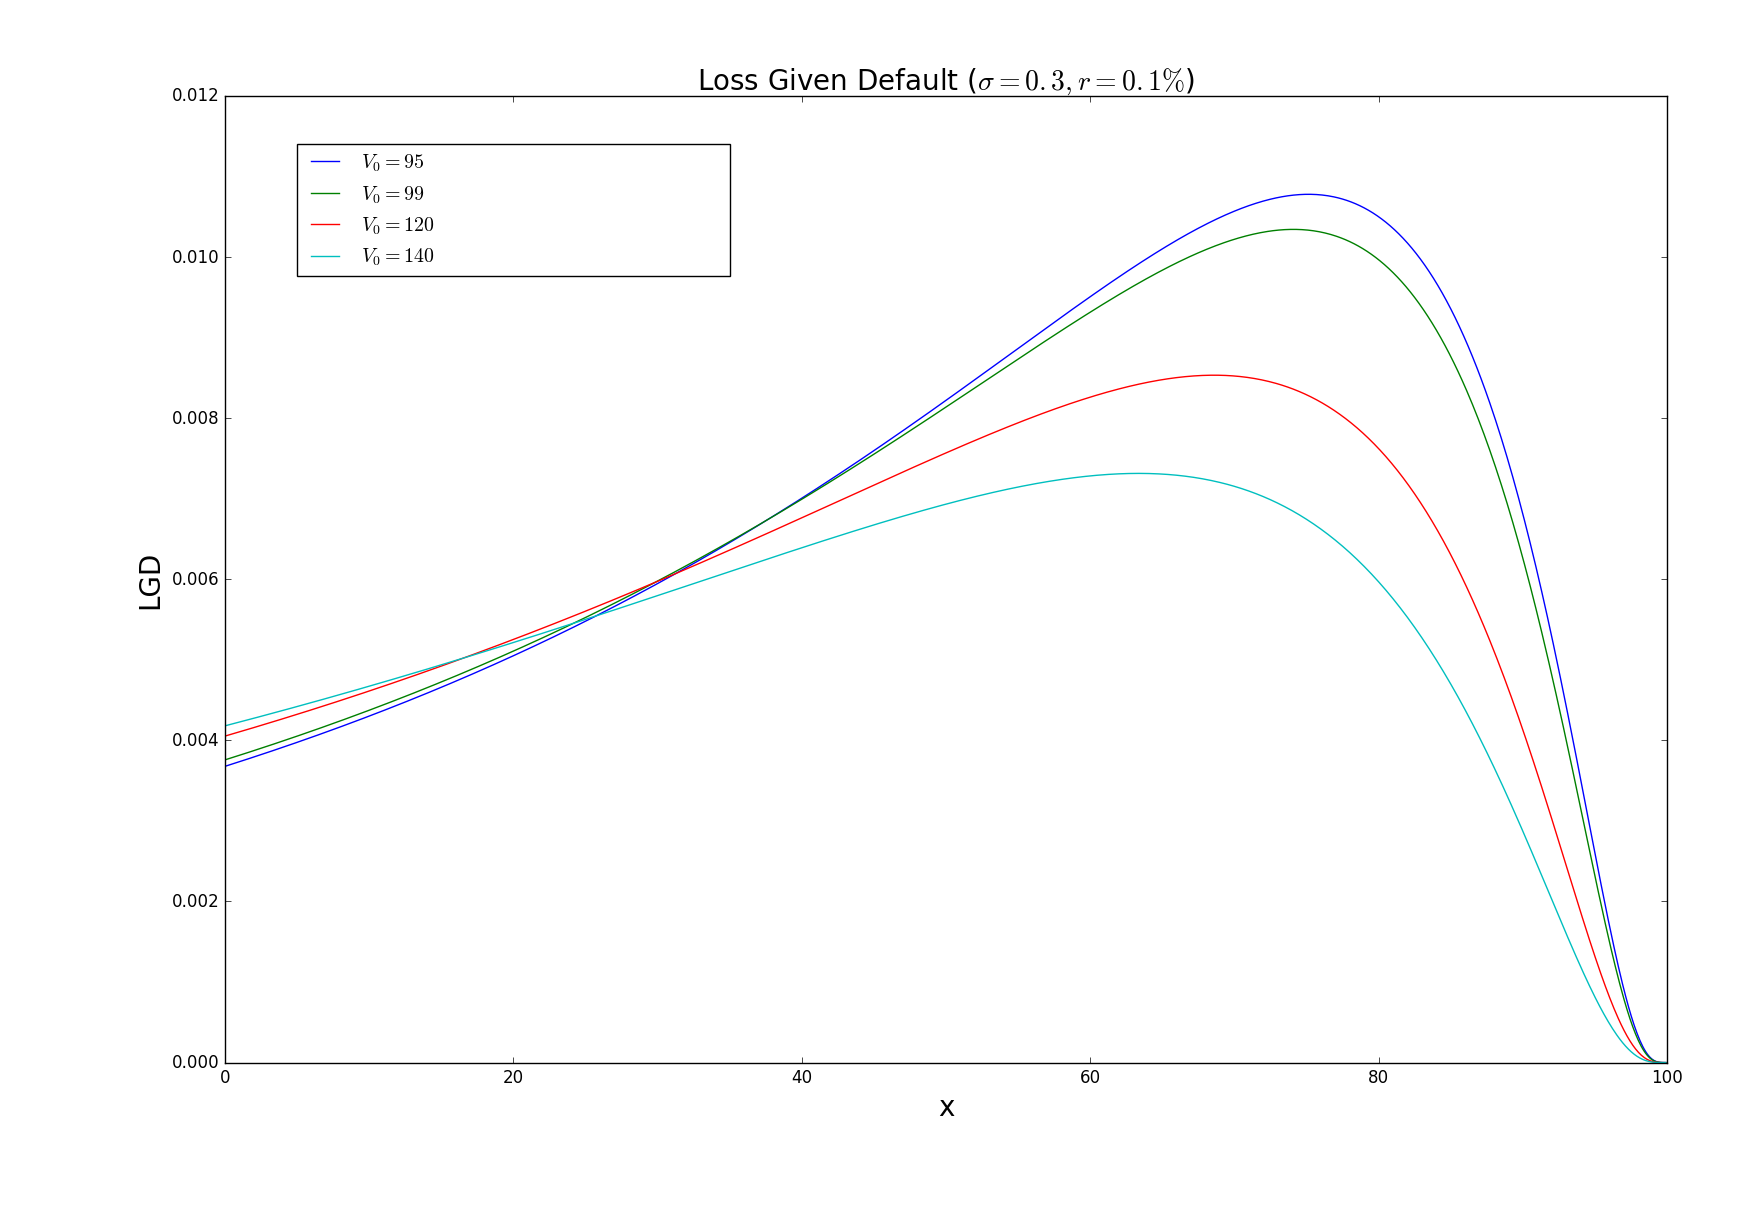
\includegraphics[width=15cm]{lgd}
\end{figure}


\newpage
\section{Recovery Value in Black-Cox Model}
Find a closed form expression for the recovery value $B^{\text{rec}}(t, T)$ in the Black
and Cox model by evaluating
$$
B^{\text{rec}}(t, T) = -\int_t^T e^{-r(s-t)}H(s)\frac{\partial}{\partial s}\Phi\left( -d(t), -d(t), -b, s-t \right)ds,
$$
where $d(t) = \frac{1}{\sigma_V}\log\frac{H(t)}{V_0}$, $H(t) = H_0 e^{at}$, $b=\frac{r-\frac{1}{2}\sigma_V^2 - a}{\sigma_V}$ and
$
\Phi(\alpha, \beta, b, t) = N\left( \frac{\alpha -bt }{\sqrt{t}} \right) - e^{2b\beta}
N\left( \frac{\alpha -2\beta -bt }{\sqrt{t}} \right).
$\\
\textit{Solution}: Given $H(t) = H_0 e^{at}$, we can write $d(t) = \frac{1}{\sigma_V} \left(\log\frac{H_0}{V_0} + at\right)$. Let $u=s-t$ in 
$$
\Phi\left( -d(t), -d(t), -b, s-t \right) = N\left( \frac{ -d(t)+b(s-t) }{\sqrt{s-t}} \right) - e^{2bd(t)}
N\left( \frac{d(t) +b(s-t) }{\sqrt{s-t}} \right),
$$
we write
\begin{align}
\nonumber B^{\text{rec}}(t, T) &= -H_0e^{at}\int_0^{T-t} e^{-(a-r)u}\frac{\partial}{\partial u}\Phi\left( -d(t), -d(t), -b, u \right)du\\
\nonumber &=-H_0e^{at}\int_0^{T-t} e^{-(a-r)u}  \left[\frac{\partial}{\partial u}N\left( \frac{ -d(t)+bu }{\sqrt{u}} \right) - e^{2bd(t)}
\frac{\partial}{\partial u} N\left( \frac{d(t) +bu }{\sqrt{u}} \right)\right] du \\
\nonumber &=-H_0e^{at}\left[\int_0^{T-t} e^{-(a-r)u}  \frac{\partial}{\partial u}N\left( \frac{ -d(t)+bu }{\sqrt{u}} \right)du - e^{2bd(t)}
\int_0^{T-t}e^{-(a-r)u}\frac{\partial}{\partial u} N\left( \frac{d(t) +bu }{\sqrt{u}} \right) du\right].
\end{align}
Denote $\tau = T-t$ and $c = a-r$, we compute
\allowdisplaybreaks
\begin{align}
\nonumber  &\quad\int_0^{\tau}e^{-c u}\frac{\partial}{\partial u} N\left( \frac{bu- d }{\sqrt{u}} \right) du\\
\nonumber 
&=   \frac{1}{2\sqrt{2\pi}}\int_0^{\tau}e^{-c u}e^{-\frac{(bu-  d)^2}{2u}} \left( \frac{b}{\sqrt{u}}+ \frac{d}{\sqrt{u^3}} \right)du \\
\nonumber &=\frac{1}{2\sqrt{2\pi}}\int_0^{\tau}e^{-\frac{2cu^2+(bu- d)^2}{2u}} \left( \frac{b}{\sqrt{u}}+ \frac{d}{\sqrt{u^3}} \right)du \\
\nonumber &=\frac{1}{2\sqrt{2\pi}}\int_0^{\tau}e^{-\frac{\left(2c+b^2\right)u^2- 2bd u + d^2}{2u}} \left( \frac{b}{\sqrt{u}}+ \frac{d}{\sqrt{u^3}} \right)du \\
\nonumber &=\frac{1}{2\sqrt{2\pi}}\int_0^{\tau}e^{-\frac{g^2 u^2- 2bd u + d^2}{2u}} \left( \frac{b}{\sqrt{u}}+ \frac{d}{\sqrt{u^3}} \right)du\\
\nonumber &\quad \text{Here denote: }  g\triangleq \sqrt{2c+b^2}\\
\nonumber &=\frac{e^{ (b\pm g)d}}{2\sqrt{2\pi}}\int_0^{\tau}e^{-\frac{\left(gu \pm d\right)^2 }{2u}} \left( \frac{b}{\sqrt{u}}+ \frac{d}{\sqrt{u^3}} \right)du \\
\nonumber &=\frac{e^{ (b\pm g)d}}{4\sqrt{2\pi}}\int_0^{\tau}e^{-\frac{\left(gu \pm d\right)^2 }{2u}} \left[     
\left( \frac{b}{g}+1 \right)  \left(\frac{g}{\sqrt{u}}+ \frac{d}{\sqrt{u^3}} \right)
+ \left( \frac{b}{g}-1 \right)  \left(\frac{g}{\sqrt{u}}- \frac{d}{\sqrt{u^3}} \right) \right]du \\
\nonumber &=\frac{e^{ (b- g)d}}{4\sqrt{2\pi}}\left( \frac{b}{g}+1 \right) \int_0^{\tau}e^{-\frac{\left(gu - d\right)^2 }{2u}}   
 \left(\frac{g}{\sqrt{u}}+ \frac{d}{\sqrt{u^3}} \right) du + \frac{e^{ (b+g)d}}{4\sqrt{2\pi}}\left( \frac{b}{g} - 1 \right) \int_0^{\tau}e^{-\frac{\left(gu+ d\right)^2 }{2u}}   
 \left(\frac{g}{\sqrt{u}}- \frac{d}{\sqrt{u^3}} \right) du \\
 \nonumber &=\frac{(b+g)e^{ (b- g)d}}{2g} \int_0^{\tau} dN\left(  \frac{gu-d}{\sqrt{u}}\right) + \frac{(b-g)e^{ (b+g)d}}{2g} \int_0^{\tau} d N\left(  \frac{gu+d}{\sqrt{u}}\right)\\
 \nonumber &=\frac{(b+g)e^{ (b- g)d}}{2g} N\left(  \frac{gu-d}{\sqrt{u}}\right)\Bigg|_{0}^{\tau} + \frac{(b-g)e^{ (b+g)d}}{2g} N\left(  \frac{gu+d}{\sqrt{u}}\right)\Bigg|_{0}^{\tau}.
\end{align}
Thus, if $d>0$,
\begin{align}
\nonumber \int_0^{\tau}e^{-c u}\frac{\partial}{\partial u} N\left( \frac{bu- d }{\sqrt{u}} \right) du
&= \frac{(b+g)e^{ (b- g)d}}{2g} N\left(  \frac{g\tau-d}{\sqrt{\tau}}\right) - \frac{(b-g)e^{ (b+g)d}}{2g} N\left(  -\frac{g\tau+d}{\sqrt{\tau}}\right)\\
\nonumber\int_0^{\tau}e^{-c u}\frac{\partial}{\partial u} N\left( \frac{bu+ d }{\sqrt{u}} \right) du
&= \frac{(b-g)e^{ -(b+ g)d}}{2g} N\left( \frac{g\tau-d}{\sqrt{\tau}}\right)-\frac{(b+g)e^{ -(b- g)d}}{2g} N\left(  -\frac{g\tau+d}{\sqrt{\tau}}\right) .
\end{align}
Back to the evaluation of $B^{\text{rec}}(t, T)$, assuming $b^2+2(a-r)>0$. If $d(t) = \frac{1}{\sigma_V} \left(\log\frac{H_0}{V_0} + at\right)>0$,
\begin{align}
\nonumber B^{\text{rec}}(t, T) &= -H_0e^{at}\left[ \frac{(b+g)e^{ (b- g)d(t)}}{2g} N\left(  \frac{g\tau-d(t)}{\sqrt{\tau}}\right) - \frac{(b-g)e^{ (b+g)d(t)}}{2g} N\left(  -\frac{g\tau+d(t)}{\sqrt{\tau}}\right) \right]\\
\nonumber &\quad +H_0e^{at+2bd(t)}\left[  \frac{(b-g)e^{ -(b+ g)d(t)}}{2g} N\left( \frac{g\tau-d(t)}{\sqrt{\tau}}\right)-\frac{(b+g)e^{ -(b- g)d(t)}}{2g} N\left(  -\frac{g\tau+d(t)}{\sqrt{\tau}}\right) \right]\\
\nonumber  &= -H_0e^{at}\left[ \frac{(b+g)e^{ (b- g)d(t)}}{2g} N\left(  \frac{g\tau-d(t)}{\sqrt{\tau}}\right) - \frac{(b-g)e^{ (b+g)d(t)}}{2g} N\left(  -\frac{g\tau+d(t)}{\sqrt{\tau}}\right) \right]\\
\nonumber &\quad +H_0e^{at}\left[  \frac{(b-g)e^{ (b- g)d(t)}}{2g} N\left( \frac{g\tau-d(t)}{\sqrt{\tau}}\right)-\frac{(b+g)e^{ (b+ g)d(t)}}{2g} N\left(  -\frac{g\tau+d(t)}{\sqrt{\tau}}\right) \right]\\
\nonumber  &= -H_0e^{at}\left[ e^{ (b- g)d(t)} N\left(  \frac{g(T-t)-d(t)}{\sqrt{T-t}}\right) +e^{ (b+g)d(t)} N\left(  -\frac{g(T-t)+d(t)}{\sqrt{T-t}}\right) \right]<0.
\end{align}
If instead $d(t) = \frac{1}{\sigma_V} \left(\log\frac{H_0}{V_0} + at\right)<0$, which is the more relevant case because $H(T)<F$,
\begin{align}
\nonumber B^{\text{rec}}(t, T) &= -H_0e^{at}\left[ \frac{(b-g)e^{ (b+ g)d(t)}}{2g} N\left( \frac{g\tau+d(t)}{\sqrt{\tau}}\right)-\frac{(b+g)e^{ (b- g)d(t)}}{2g} N\left(  -\frac{g\tau-d(t)}{\sqrt{\tau}}\right) \right]\\
\nonumber &\quad +H_0e^{at+2bd(t)}\left[  \frac{(b+g)e^{ -(b- g)d(t)}}{2g} N\left(  \frac{g\tau+d(t)}{\sqrt{\tau}}\right) - \frac{(b-g)e^{ -(b+g)d(t)}}{2g} N\left(  -\frac{g\tau-d(t)}{\sqrt{\tau}}\right) \right]\\
\nonumber &= -H_0e^{at}\left[ \frac{(b-g)e^{ (b+ g)d(t)}}{2g} N\left( \frac{g\tau+d(t)}{\sqrt{\tau}}\right)-\frac{(b+g)e^{ (b- g)d(t)}}{2g} N\left(  -\frac{g\tau-d(t)}{\sqrt{\tau}}\right) \right]\\
\nonumber &\quad +H_0e^{at}\left[  \frac{(b+g)e^{ (b+ g)d(t)}}{2g} N\left(  \frac{g\tau+d(t)}{\sqrt{\tau}}\right) - \frac{(b-g)e^{ (b-g)d(t)}}{2g} N\left(  -\frac{g\tau-d(t)}{\sqrt{\tau}}\right) \right]\\
\nonumber &=H_0e^{at}\left[  e^{ (b-g)d(t)} N\left(  -\frac{g(T-t)-d(t)}{\sqrt{T-t}}\right) +  e^{ (b+ g)d(t)} N\left(  \frac{g(T-t)u+d(t)}{\sqrt{T-t}}\right) \right]>0.
\end{align}
where $g\triangleq \sqrt{b^2+2(a-r)}$.

\newpage

\section{Cox Process with Normal Intensity}
Consider the Cox model where the intensity follows the normal process
$$
d\lambda(t) = \theta dt +\sigma dW(t),
$$
with constant $\theta$ and $\lambda(t=0)=\lambda_0$.

\textbf{(i) }Calculate the survival probability $S(0,t)$ for this Cox process.

\textit{Solution}: Integrate the normal process,
$ \lambda(t) = \lambda_0+ \theta t + \sigma W(t)$.
Integrate again with respect to time,
\begin{align}
\nonumber \int_0^t \lambda(s)ds = \lambda_0 t + \frac{1}{2}\theta t^2 + \sigma\int_0^t W(s)ds
\sim N\left(\lambda_0 t + \frac{1}{2}\theta t^2, \frac{1}{3}\sigma^2 t^3\right),
\end{align}
where the stochastic version of Fubini's thoerem is used to compute the probability distribution of the integral $\int_0^t W(s)ds$. The survival probability
\begin{align}
\nonumber S(0,t) &\triangleq \mathbb{E}\left[e^{-\int_0^t \lambda(s)ds}\right]\\
\nonumber &= \mathbb{E}\left[e^{- \lambda_0 t - \frac{1}{2}\theta t^2 - \sigma\int_0^t W(s)ds }\right]\\
\nonumber &= e^{- \lambda_0 t - \frac{1}{2}\theta t^2 +\frac{1}{6}\sigma^2 t^3 },
\end{align}
where we have used $\mathbb{E}\left[e^{-X}\right]=e^{-\mathbb{E}[X]+\frac{1}{2}\text{Var}[X]}$ for a normal variable $X$.\\

\textbf{(ii)} Design and implement an algorithm for simulating events from
this Cox process.
\begin{lstlisting}
import math
import numpy as np
print("-------------------------")
print("Simulation of Cox Process")
print("-------------------------")
# input parameters
lambda0 = 0.03  # initial intensity
theta = 0.005  # intensity drift
sigma = 0.008  # intensity diffusion
t = 10.0  # time horizon
ns = 1000000  # number of samples
dt = 0.001  # time step width
timer = np.array([1,2,3,4,5,6,7,8,9,10])  # time points to record counts
     
# derived parameters
n = int(t/dt)  # time step number
dt_root = math.sqrt(dt)  # square root of time step
theta_dt = theta*dt      
indexer = (timer/dt).astype(int);
m = len(timer)
stats = np.zeros(m)

# simulation
for k in range(ns):
    timesteps = np.zeros(n+1)
    lambdas = np.zeros(n+1)
    lambdas[0] = lambda0
    counts = np.zeros(n+1)
    for i in range(n):
        # march forward in time
        timesteps[i+1] = timesteps[i] + dt
        # generate intensity process 
        normal = np.random.normal(0, dt_root)
        lambdas[i+1] = lambdas[i] + theta_dt + sigma*normal
        # generate counting process
        lambda_dt = lambdas[i+1]*dt
        uniform = np.random.random()
        if uniform <= lambda_dt: counts[i+1] = counts[i]+1
        else: counts[i+1] = counts[i]
        
    # generate statistics
    for i in range(m):
        if counts[indexer[i]] > 0:
            stats[i] += 1
\end{lstlisting}

\textbf{(iii)} Verify the correctness of your algorithm by comparing the estimated survival
probabilities with the closed form formula. Use $\lambda_0=0.03$, $\theta=0.005$, 
$\sigma=0.008$, and a range of values of $t$, say $t=1,2,\cdots, 10$.\\
\textit{Solution}: We sample a number $N_s = 1,000,000$ of $\lambda(t)_{0\le t\le T}$ paths and simulate
the counting process conditioned on each $\lambda(t)$ path. The width of each time step
is chosen to be $\Delta t = 0.001$. The results are reported in the following table. 
The column "Hit Events" records the number of
sample paths that end up with a default, and the vice versa for column "Miss Events".
The estimated survival rates (ratio of Miss Events and $N_s$) tabulated in the column "$S(0,t)$ Estimate" match the theoretical
values of the survival rate up to the third significant digits. Using a coarser time step $\Delta t=0.01$
yields the same level of accuracy with $1,000,000$ sample paths. This indicates that the cause 
of the error is primarily statistical $\sim\frac{1}{\sqrt{N_s}}\approx 0.001$.
\begin{center}
{
\pgfplotstabletypeset[
    col sep=comma,
    string type,
    columns/natural/.style={column name=natural, column type={|l}},
    columns/two/.style={column name=two, column type={|l}},
    columns/three/.style={column name=three, column type={|c|}},
    every head row/.style={before row=\hline,after row=\hline},
    every last row/.style={after row=\hline},
    ]{results.csv}
}
\end{center}


\end{document}